%\RequirePackage{plautopatch} % パッチを自動的に適用してくれる

% 仕様 ----------------------------------------------------------------------------------------------------------------

\documentclass[b5paper,11pt,dvipdfmx]{jsarticle}
\usepackage{amsmath,amssymb,amsthm,amsfonts}
\usepackage{hyperref}
\usepackage{mathtools}
\usepackage{graphicx}
\usepackage{url}
\usepackage{calligra}
\usepackage{physics}
\usepackage{tikz}
\usepackage{tcolorbox}
\usepackage{mathcomp}
\usepackage{textcomp}
\usepackage{pxjahyper}

\numberwithin{equation}{section}
\theoremstyle{definition}
\newtheorem{thm}{定理}[section]
\newtheorem{lem}[thm]{補題}
\newtheorem{prop}[thm]{命題}
\newtheorem{cor}[thm]{系}
\newtheorem{ass}[thm]{仮定}
\newtheorem{conj}[thm]{予想}
\newtheorem{dfn}[thm]{定義}
\newtheorem{rem}[thm]{注}


% 追加するパッケージたち ----------------------------------------------------------------------------------------------------------------

\usepackage{mathrsfs} % 花文字をいれる
\usepackage{bm,ascmac,latexsym,color}
\usepackage{varwidth}
\usepackage{pxrubrica}
\usepackage{titlesec}
\usepackage{tocloft}
\hypersetup{
    colorlinks=true,
    %linkcolor=red,
    %citecolor=green,
    %urlcolor=magenta
    }

\usetikzlibrary{calc}
\tcbuselibrary{raster,breakable,theorems,skins}


% プリアンブルおわり ==============================================================

\begin{document}

\title{ホログラフィック超伝導の進展から}
\author{広島大学 素粒子ハドロン研究室 川合玲央}
\date{}

\maketitle

%\tableofcontents

\begin{abstract}
    本記事ではホログラフィー原理による超伝導現象の解析の試みと,特にその近年の進展について紹介します.
    ホログラフィー原理とは重力理論とゲージ理論が等価であるという主張であり,
    量子重力理論の構築への足がけとして期待されている枠組みです.
    そんな熱い期待\footnote{筆者の主観です.}がかけられているホログラフィー原理は,実はその端緒を弦理論にもちます.
    にもかかわらず弦理論がよく言われる検証不可能性
    \footnote{弦理論の典型的なエネルギースケールは$10^{19}$GeV程度であり,
    現在稼働している加速器のエネルギースケールは$10^4$GeV程度です.
    かなりの差がありますね.この事実をもってして弦理論は現実的な観点から検証不可能であると言われたりすることがあります.
    ただ高エネルギースケールの弦理論から示唆される結果は,
    弦理論それ自体の検証ができなくとも我々がよく知っている現実的なスケールの物理も含んでいると期待しているわけですから,
    それら低エネルギー有効理論に対する制限を与えるなど多くの場面で有用です.
    ホログラフィー原理もその一種だと筆者は思っています.
    またstring phenomenologyという分野もあると聞きますが,筆者はその有用性と詳細を知らないのでこれには言及しません.}
    にとらわれず,実際に現実の観測量と結びつける研究が多数行われています.
    よく挙げられる例としてはクォーク・グルーオン・プラズマ\cite{Policastro01,Kovtun04}
    や超伝導\cite{Hartnoll08a,Hartnoll08b}があります.
    特に超伝導に関しては近年大きな発展があり,
    ホットトピックと言えると思います\footnote{筆者の主観です.},
    ということで今回は超伝導(正確には超伝導っぽいもの)のホログラフィー原理を用いた解析を見ていきましょう.
\end{abstract}


\section{ホログラフィー原理}
皆さんはホログラフィー原理,もしくはAdS/CFT対応という言葉を聞いたことがあるでしょうか?
AdS/CFT対応ともよばれ,$d + 2$次元の重力理論と$d + 1$次元のゲージ理論が等価になるという主張です.
1997年にMaldacenaにより最初の例が示されました\cite{Maldacena97}.
以降多くの論文が弦理論の主戦場であるhep-thに限らず様々な分野で投稿されています.
ここではそのホログラフィー原理に関して簡単に概観していこうと思います
\footnote{ページ数と筆者の力不足によりほとんどお話になっています.
真面目に議論と計算を追うなら\cite{Witten98,Aharony99,Bousso02,Ammon15}あたりを参照してください.}.

ホログラフィー原理は超弦理論における閉弦と開弦の間にある双対性から示唆される対応関係です.
弦理論はその名の通り,1次元の自由度をもつ弦を基本的対象とする理論のことで,
0次元の質点からなる従来の素粒子理論から自由度が増えている分,様々なことを表現できるようになります.

素粒子物理学における一つの目的はすべての事象を説明するような統一理論の構築にあるでしょう.
しかし現状の理論では4つある基本相互作用のうち重力とそれ以外の相互作用についての理論を
うまく整合して組み合わせることができていません
\footnote{重力の量子化がこれまでの手法ではうまくいかないことに起因します.
ここではこれ以上触れませんが,歴史を含めたこれに関する話題は\cite{Yoneya21}が詳しいと思います.}.
現在明確な実験事実等はないものの,これを解決する統一理論として超弦理論は期待されています.
ということは我々の知っている物理は弦理論に低エネルギー有効理論として含まれているはずです.


弦には両端がつながっている閉弦と両端がつながっていない開弦があり,
これらの低エネルギー有効理論はそれぞれ重力理論とゲージ理論です.

Dブレーンという対象を通じて閉弦と開弦は対応していると考えられており,
低エネルギー有効理論の間にもその対応関係がある


証明はないものの,多くの
例が計算され,
\begin{figure}[t]
    \centering
    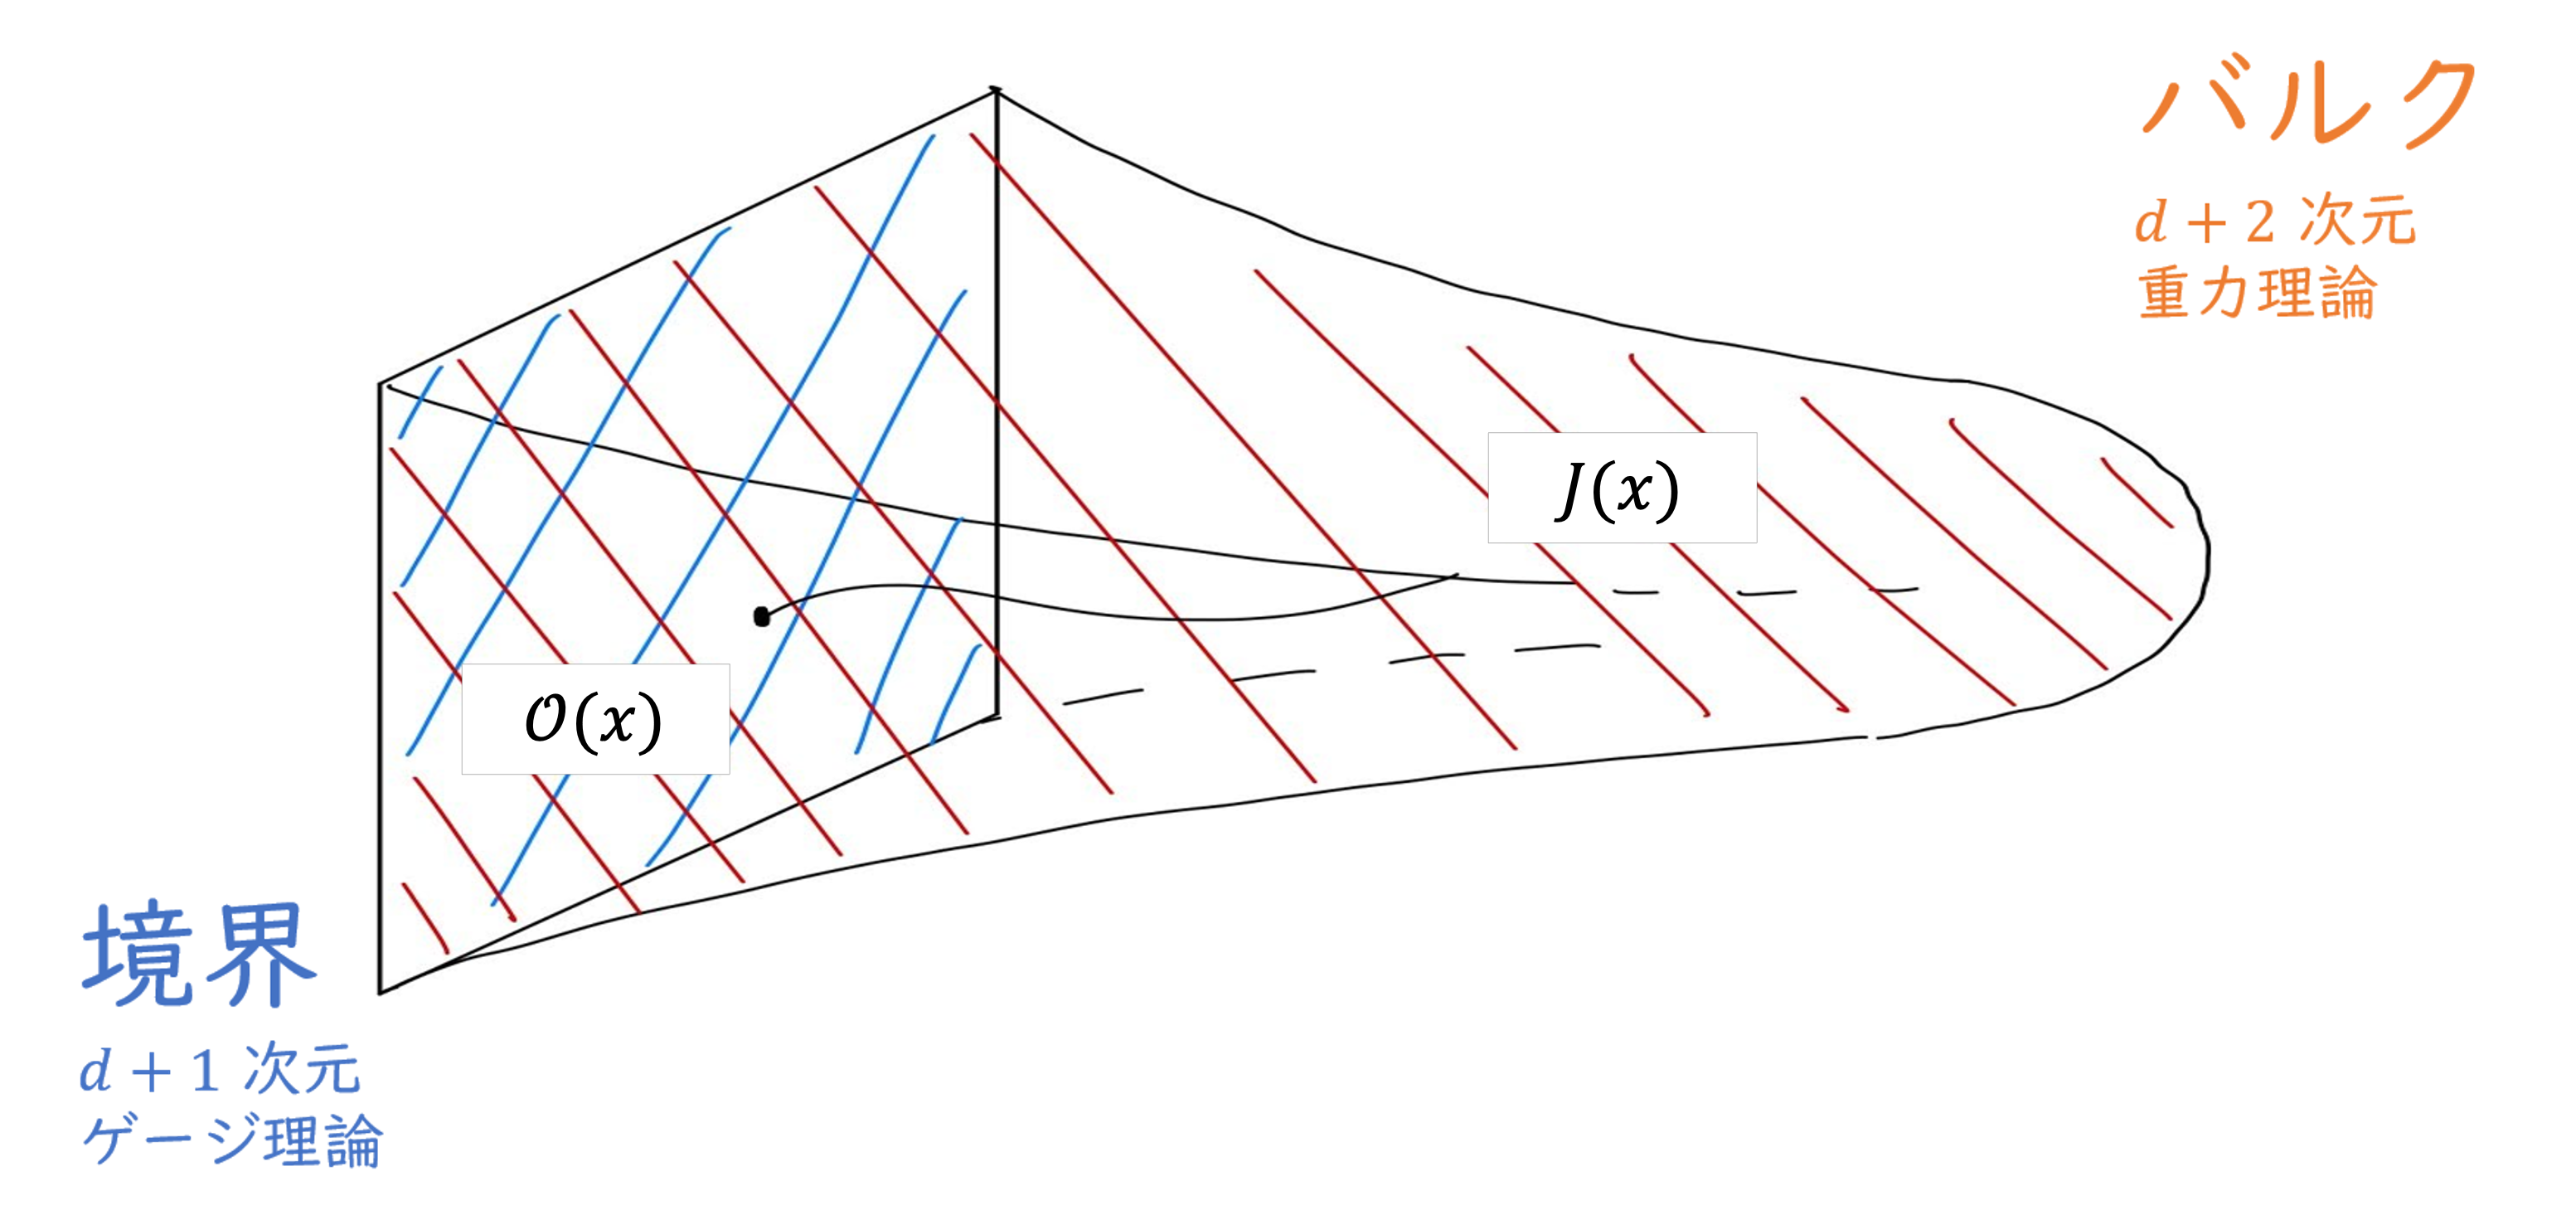
\includegraphics[width=0.9\textwidth]{holography.png}
    \caption{ホログラフィー原理の概念図}
    \label{fig:holography}
\end{figure}

具体的な対応関係として
GKP--Witten関係式\cite{Gubser98,Witten98}

\begin{equation}
    \exp(i S_{\text{tot}}[J])
    = \ev{\exp\left[ i \left( S_{\text{YM}}
    + \int \dd^{p+1} x \mathcal{J}(x) \mathcal{O}(x) \right)\right]}
\end{equation}

バルク中の場$\mathcal{J}(x)$が境界上の物理量$\mathcal{O}(x)$のソースとなる




\subsection{クォーク・グルーオン・プラズマ}
ここでホログラフィー原理が話題
契機となった代表的な例の話をしておきましょう.

Brookhaven National Laboratoryの加速器Relativistic Heavy Ion Colliderで


弦理論による「予言」が
実験結果$\frac{\eta}{s} \approx 0.1$,
ホログラフィーによる計算$\frac{\eta}{s} = \frac{1 \hbar}{4 \pi k_B} \approx 0.08$.

実際にその実験レポート\cite{PHENIX06}では




引用されている粘性の「予言」\cite{Kovtun04}

このようにクォーク・グルーオン・プラズマにおける「成功」があり,
他の例への応用もより精力的に研究されるようになりました.
その一例が今回紹介する超伝導です.


\section{ホログラフィック超伝導}

\subsection{高温超伝導}
\begin{figure}[t]
    \centering
    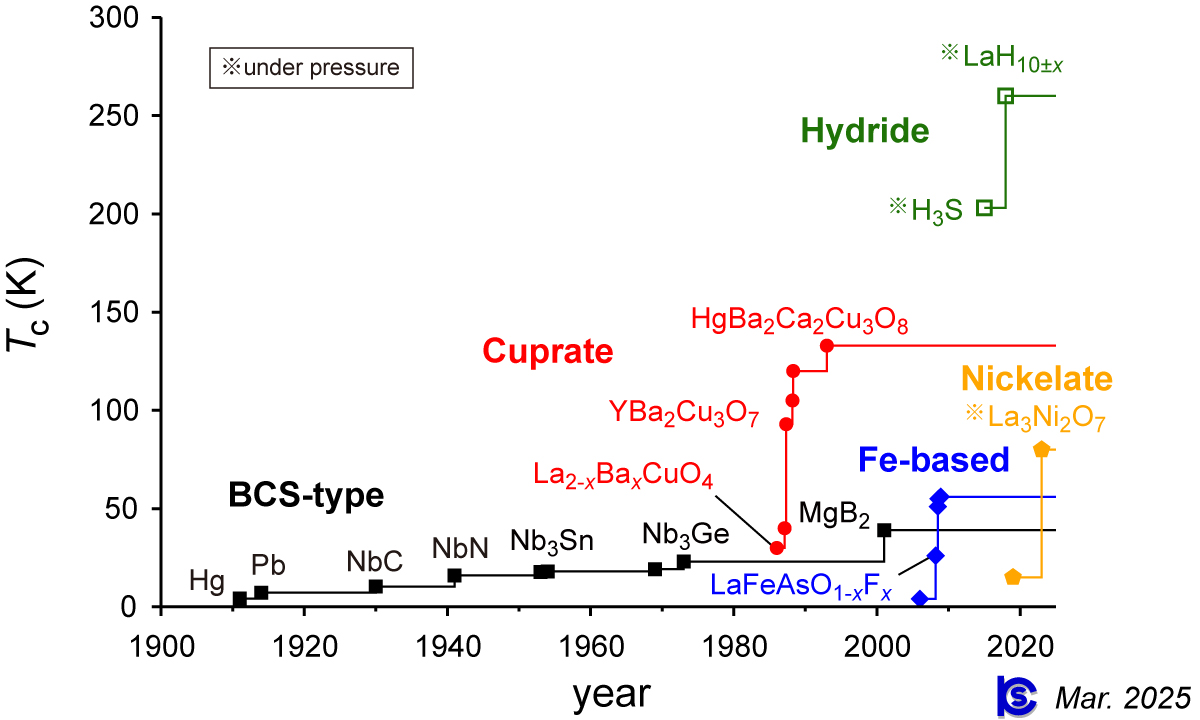
\includegraphics[width=0.9\textwidth]{tc-history_2025.jpg}
    \caption{超伝導転移温度の記録}
    \label{fig:tc-history}
\end{figure}
%東京大学 大学院総合文化研究科 広域科学専攻 相関基礎科学系 橘高研究室
%\url{https://park.itc.u-tokyo.ac.jp/kittaka/contents/others/tc-history/index.html}


とりあえず同じような強結合の場に応用してみる
物性においてはそのような強相関系

中村真の仕事で、時間依存する重力時空と流体力学の関係、および時空の正則性と
流体の輸送係数を論じた代表的な論文は
S. Kinoshita, S. Mukohyama, S. Nakamura and K. y. Oda, “Consistent Anti-de
Sitter-Space/Conformal-Field-Theory Dual for a Time-Dependent Finite Tem-
perature System,” Phys. Rev. Lett. 102 (2009) 031601 [arXiv:0901.4834 [hep-
th]];
S. Kinoshita, S. Mukohyama, S. Nakamura and K. y. Oda, “A Holographic
Dual of Bjorken Flow,” Prog. Theor. Phys. 121 (2009) 121 [arXiv:0807.3797
[hep-th]].
なお、これら一連の仕事の発端となった研究は、
R. A. Janik and R. B. Peschanski, “Asymptotic perfect fluid dynamics as
a consequence of AdS/CFT,” Phys. Rev. D 73, 045013 (2006) [arXiv:hep-
th/0512162].




解析手段としてのホログラフィー原理
→ RHICにおける成功
• その他の強結合ゲージ場への応用
→ 高温超伝導に対する期待
• ホログラフィック超伝導にあった問題点の解決
→ 境界上の電磁場にダイナミクスを導入



ホログラフィック超伝導というのがあるよ

強結合、つまり高温超伝導を解決できるかもしれないよ

ホログラフィーっていうのは場の理論の問題を重力を使って簡単に解くことができる手法だよ

従来のホログラフィック超伝導はゲージ場がダイナミカルじゃないから問題だよ
(例えばMeissner効果が起きないよ???)

最近提唱されたモデルではMeissner効果が起きるなど従来の問題を解決したよ




















\clearpage


Hartnollのレビュー!!!!!!!!!!!!!!!!!!!!!!

厳密にはマイスナー効果は起こらないが
マイスナー効果を引き起こすための本質的な物理
London方程式は導出されている

なぜ厳密には起こらないのか?

HHH論文自身が明確に述べている通り、このモデルでは電流が電磁場を生み出さないため、
厳密な意味でのマイスナー効果は存在しえません
マイスナー効果とは、超伝導体内部に生じた電流が、
外部磁場を打ち消すような逆向きの磁場を「自ら」作り出すことで磁場を排除する現象
電流が磁場を生み出せない設定である以上、この現象は起こり得ません 。

HHH論文の非常に重要な功績は、このモデルを用いて
ロンドン方程式 $J_i = -n_s A_i$ を導出したことです
ロンドン方程式は、ベクトルポテンシャル$A_i$ が存在するだけで(つまり磁場が存在するだけで)
電流 $J_i$ が流れることを示す、超伝導の根幹をなす関係式です 。
著者らは、このロンドン方程式が成立することを示した上で、
「もしこの理論を(後から)弱くゲージ化して、電流がマクスウェル方程式に従って磁場を生み出すようにすれば、
磁場は排除されるだろう」と論じています 。

つまり、HHH論文のモデルは、マイスナー効果という「現象」そのものは示しませんが
その現象を引き起こす原因である「ロンドン方程式」が、
このホログラフィックなセットアップから自然に導出されることを初めて示したのです。










新旧の違い!!!!!!!!!!!!!!!!!!!!!!!

従来模型 (HHH論文):

境界でのU(1)対称性はグローバル対称性
境界の電磁場(光子)が力学(ダイナミクス)を持たず外部から固定された**「外部ソース」**としてのみ存在

このモデルでは、外部からかけた電磁場に対して物質(超伝導体)がどのように応答し、
どんな電流$\langle J \rangle$ が流れるかを計算します。
しかし、その電流が電磁場自体にフィードバックを与える効果は、モデルの内部では考慮されません 。

新規模型 (Natsuume論文):
境界での電磁場を
ダイナミカルな場として扱います 。
これを実現するために、「半古典的なマクスウェル方程式 ($\nabla F = e^2 \langle J \rangle$)」
そのものを境界条件として課します 。
これにより、物質が生み出す電流 $\langle J \rangle$ が、電磁場 $F$ を変化させるという
バックリアクションがモデルに最初から組み込まれています。

従来模型が「固定された磁場に物質がどう応答するか」を見るのに対し、
新規模型は「磁場と物質が互いに影響を及ぼしあう、自己無撞着な状態」を直接解いている













\section{より現実的なモデルにするために}

上で作った模型は現実の超伝導の解析という目的からすると多くの問題があります.
\begin{itemize}
    \item Meissner効果が起こらない
    \item ラージNゲージ理論になっている
    \item AAA
\end{itemize}
ここでは
のMeissner効果が起こらないについて

作用にはMaxwell場が入っているじゃないかと思われるかもしれませんが,

Natsuume論文の新規模型は、HHH論文などで確立された従来模型の「外部ソース」という制限を取り払い、
電磁場のダイナミクスを直接組み込むことで、従来は間接的にしか示唆できなかったマイスナー効果を、
モデル内で直接的かつ解析的に示すことに成功した

\subsection{ホログラフィックMeissner効果}




\subsection{5次元模型}

ホログラフィック繰り込みの考えから境界に対数項$S_{\text{ct}}$が必要となる.
オンシェル超重力作用$S_{\text{sugra}}$の発散は、
バルク時空の境界(カットオフ$\rho = \epsilon$または$r^2 = \epsilon$)で評価されますが、その発散の構造は境界次元$d$に依存します。
• 奇数次元の場合: 発散項は$\epsilon$の逆べき乗($\frac{1}{\epsilon^k}$)の形のみで出現します。
• 偶数次元の場合: $\epsilon$の逆べき乗の項に加えて、対数発散項$\log \epsilon$が出現します


対数発散は、ホログラフィック繰り込みにおいて特殊な対処を必要とします。

作用を有限化するためには、この$\log$の発散も打ち消すように、
境界対項$S_{ct}$を含めなければなりません\cite{deHaro00}.






夏梅のレビュー!!!!!!!!!!!!!!!!!

超伝導らしきものを再現するための作用
s波ホログラフィック超伝導

理論モデル
4(5)次元時空(バルク)中のアインシュタイン・マクスウェル・スカラー理論
ホログラフィック超伝導体を記述する標準的なモデル
背景時空
バルクの時空は、ブラックホールが存在するSchwarzschild-AdS$_4$(5)時空
このブラックホールのホーキング温度が、境界の(2+1)(3+1)次元時空の温度に対応

\begin{equation}
    \begin{split}
        S_{\text{bulk}}
        &= \int \dd^4 x \sqrt{-g} \left( \mathcal{L}_g + \mathcal{L}_{\text{matter}} \right)\\
        \mathcal{L}_{g}
        &= R - 2 \Lambda\\
        \mathcal{L}_{\text{matter}}
        &= - \frac{1}{g^2} \left( \frac{1}{4} F^{MN} F_{MN} + |D_M \Psi|^2 + m^2 |\Psi|^2 \right)
    \end{split}
\end{equation}

ただし
\begin{equation}
    \begin{split}
        F_{MN} &= \partial_M A_N - \partial_N A_M,\\
        D_M &= \nabla_M - i A_M,\\
        \Lambda &= - \frac{3}{L^2}.
    \end{split}
\end{equation}

Maxwell場およびスカラー場が重力場と結合しない.
解析を簡単にするためにプローブ近似
$g \gg 1$ (or $q \to \infty$)
をとることで物質場から重力への影響・バックリアクションを無視できるようにする.

運動方程式は
どうこう

$A_u = 0$のゲージをとる
運動方程式は
どうこう

物質場の漸近的振る舞いは
\begin{equation}
    \begin{split}
        A_\mu &\sim \mathcal{A}_\mu+A_\mu^{(+)} u,\\
        \Psi &\sim \Psi^{(-)} u^{\Delta_{-}}+\Psi^{(+)} u^{\Delta_{+}},\\
        \Delta_{\pm} &\coloneq \frac{3}{2} \pm \nu, \quad \nu = \sqrt{\frac{9}{4}+m^2}.
    \end{split}
\end{equation}

\begin{equation}
    \begin{split}
        \ev{\mathcal{J}_\mu} &= \left.\frac{1}{g^2} F_{u \mu}\right|_{u=0} \\
        \ev{\mathcal{O}} &=\frac{1}{g^2} 2 \nu \Psi^{(+)}.
    \end{split}
\end{equation}

AdS/CFT辞書: バルクの場の境界近く($u \to 0$)での振る舞いが、境界の物理量に対応します。

バルクのベクトルポテンシャル
$A_\mu$の境界値$\mathcal{A}_\mu$が境界のベクトルポテンシャル
$A_\mu$の次のオーダーの項$A_\mu^{(+)}$が境界の電流$\ev{\mathcal{J}_\mu}$に対応する



バルクのスカラー場
$\Psi$の境界での主要項$\Psi^{(+)}$が超伝導の秩序パラメータ$\ev{\mathcal{O}}$に対応する


$\mathcal{A}_t = \mu$は化学ポテンシャルを
$A~{(+)}_t$は荷電密度$\ev{\rho}$を
同様に$\mathcal{A}_i$はベクトルポテンシャルを
$A^{(+)}_i$はカレント密度$\ev{\mathcal{J_i}}$を
$\Psi^{(+)}$はオーダーパラメータ$\ev{\mathcal{O}}$を
$\Psi^{(-)}$はオーダーパラメータの外場ソースを表す



Section III: Small Magnetic Field (小さい磁場をかけた場合)
ここがこの論文の最初の核心部分です。一定の超伝導状態に、弱い磁場をかけてみて、その応答を調べることでマイスナー効果を解析します。

A. Dirichlet Boundary Condition (通常の境界条件)
まず、従来の手法、つまり境界の電磁場
$\mathcal{A}_\mu$ を固定するディリクレ境界条件で計算するとどうなるかを見ています 。


計算: バルクのマクスウェル方程式 (3.2)  を解くと、境界での電流
$\ev{\tilde{\mathcal{J}}_y}$ は、境界のベクトルポテンシャル $\tilde{\mathcal{A}}_y$ を用いて
次のように書けることを導出します($q$ は運動量)。

\begin{equation}
    \begin{split}
        \ev{\tilde{\mathcal{J}}_y}& =\left.\partial_u \tilde{A}_y\right|_{u=0} \\
        & =\tilde{\mathcal{A}}_y\left(-q^2-2 \int_0^1 d u\left|\varphi_0\right|^2+\cdots\right)
    \end{split}
\end{equation}
電流は2つの部分からなる
超電流
$-2\int |\varphi_0|^2$ の項は、超伝導電子による電流ですこれはロンドン方程式に対応
束縛電流
$-q^2$の項は超伝導凝縮がない($\varphi_0=0$)通常の状態でも存在する電流
論文ではこれが物質の磁化による束縛電流として解釈できると指摘
境界のマクスウェル方程式(アンペールの法則)が存在しないため
(境界条件として電流が存在するだけで、Maxwell場はダイナミカルに存在はしない)
超電流が磁場を押し返すことができず、マイスナー効果は起こりません
磁場は超伝導体内部に自由に侵入できてしまいます

元の境界条件
$\mathcal{A}_\mu = \left. A_\mu \right|_{u = 0}$






新たな境界条件
非自明な解をとるために外場ソース$\mathcal{J}_{\text{ext}}^i$を加えてやる
\begin{equation}
    \partial_{j} \mathcal{F}^{ij}
    = e^{2} \left( \ev{\mathcal{J}^{i}} + \mathcal{J}_{\text{ext}}^i \right)
\end{equation}

\begin{equation}
    q^2 \tilde{\mathcal{A}}_y
    = \frac{e^2}{1 + e^2} \tilde{\mathcal{J}}^{\text{ext}}_y
    \coloneq \mu_m \tilde{\mathcal{J}}^{\text{ext}}_y
\end{equation}







\begin{equation}
    \begin{split}
            \mu_m
            &= \frac{e^2}{1 + e^2 / r_0}\\
            \chi_m
            &= - \frac{e^2 / r_0}{1 + e^2 / r_0}\\
            \lambda^2
            &= \frac{1 + e^2 / r_0}{2 e^2 I}\frac{1}{r_0}
    \end{split}
\end{equation}


















各種表式を代入してやり,Fourier変換などをいろいろして解く(方程式を出す)



結果の話

Meissner効果
\begin{equation}
    \mathcal{A}_{y}\propto e^{-x/\lambda}
\end{equation}
$\lambda$は磁場侵入長

境界での電流には、超伝導電子による
超電流の他に、物質の磁化に由来する束縛電流 (bound current) が存在する
束縛電流の効果により、物質の透磁率$\mu_m$ が真空の値からずれ,物性が変化

極端な第一種超伝導体にはなれない:

通常のギンツブルグ・ランダウ(GL)理論では、結合定数$e$を大きくすると
$e\rightarrow\infty$ で磁場侵入長がゼロ $\lambda \to 0$ となり、
磁場を完全に排除する極端な第一種超伝導体になります
しかし、このホログラフィックなモデルでは、束縛電流の効果により
$e\rightarrow\infty$ としても $\lambda$ が有限の値を保ち、極端な第一種にはなれないことが示されました

GLパラメータの導出(5次元バルクの場合):
特に解析的な解が得られる5次元バルクのモデルにおいて、磁場侵入長$\lambda$とコヒーレンス長 $\xi$ を具体的に計算し、
超伝導体の種類(第一種か第二種か)を決定するGLパラメータ $\kappa^2 = \lambda^2 / \xi^2$ を解析的に導出
超伝導体の性質が温度や結合定数にどう依存するかが明らかになりました









\clearpage


%======================================================================
\section{ホログラフィー原理とは何か?}
%======================================================================

ホログラフィー原理を一言で表すなら,「物理法則はホログラムのようになっている」という主張です.
皆さんがご存知のホログラムは,2次元のフィルムに3次元の立体像の情報を全て書き込んだものです.
これと同じように,ホログラフィー原理は,「ある次元の重力を含む物理理論」が,「それより1次元低い,重力を含まない場の量子論」と完全に等価であると主張します.

この一見奇妙な対応関係は,AdS/CFT対応\cite{Maldacena97}という形で定式化されています.
これは,バルク(bulk)と呼ばれる$d+1$次元の反ド・ジッター(AdS)時空\footnote{
AdS時空とは,負の宇宙項を持つアインシュタイン方程式の真空解です.我々の宇宙が正の宇宙項を持ち加速膨張しているのとは対照的に,AdS時空は全体が内側に曲がった双曲的な構造をしています.
}における重力理論が,その時空の境界(boundary)にある$d$次元の共形場理論(CFT)\footnote{
共形場理論とは,スケール変換に対して対称性を持つ場の量子論のことです.素粒子物理学だけでなく,物性物理学における相転移など,様々な場面に現れる普遍的な理論です.
}と等価である,というものです.

\begin{figure}[h]
    \centering
    % \includegraphics[width=0.6\linewidth]{AdS_CFT.png} % 画像ファイルがある場合
    \framebox[0.6\linewidth][c]{ここにAdS/CFTの模式図(円筒とその内部)を挿入}
    \caption{AdS/CFT対応の模式図.円筒の内部(バルク)の重力理論が,円筒の表面(境界)の場の量子論と等価になる.}
    \label{fig:adscft}
\end{figure}

この対応の何が強力かというと,2つの理論の「結合の強さ」が逆転する点にあります.
境界の場の量子論が,計算が非常に難しい「強結合」の状態にあるとき,バルクの重力理論は,アインシュタイン方程式などを解けばよい「弱結合(古典)」の状態に対応します.
つまり,我々がこれまで歯が立たなかった強結合な量子多体系の問題を,得意な一般相対性理論の計算に「翻訳」して解くことができるのです.
この翻訳ルールは「AdS/CFT辞書」と呼ばれ,2つの理論の物理量を結びつけます.
この強力な計算ツールを用いて,物性物理学の難問である「超伝導」に挑んだのが,ホログラフィック超伝導です.

\clearpage

%======================================================================
\section{ホログラフィック超伝導の従来模型}
%======================================================================

ホログラフィック超伝導の最初の具体的なモデルは,Hartnoll, Herzog, Horowitzによって2008年に提案されました\cite{Hartnoll08a, Hartnoll08b}.
彼らは,超伝導という現象をホログラフィーで記述するための,いわば「最小構成(ミニマルモデル)」を考えました.

\subsection{モデルの構成要素}

まず,我々が住む世界の超伝導体(境界の理論)で必要なものは何でしょうか.
それは,電荷を担う電子対(クーパー対)が一斉に同じ量子状態に落ちる「凝縮」という現象です.
これを記述するためには,
\begin{itemize}
    \item U(1)グローバル対称性(電荷の保存に対応)
    \item 電荷をもち,凝縮する演算子 $\mathcal{O}$
\end{itemize}
の2つがあれば十分です.AdS/CFT辞書によれば,これらはバルクの重力理論において,
\begin{itemize}
    \item マクスウェル場 $A_a$
    \item 電荷$q$を持つスカラー場 $\psi$
\end{itemize}
にそれぞれ対応します.これらをアインシュタイン重力と組み合わせた「アインシュタイン・マクスウェル・スカラー理論」が,ホログラフィック超伝導の舞台となります.

\subsection{超伝導への相転移}

このモデルでは,バルクに電荷を持つブラックホールを考えます.
ブラックホールのホーキング温度が,境界の超伝導体の温度に対応します.
高温状態では,ブラックホールはスカラー場をまとっておらず,「毛のない(bald)」状態です.
これは境界の理論が常伝導状態にあることに対応します.

ところが,温度を下げていくと,ある臨界温度$T_c$でブラックホールは不安定になり,スカラー場$\psi$がブラックホールの周りに発生します.
これを「スカラーの毛が生えた(hairy)」ブラックホールと呼びます\cite{Hartnoll08a}.
このスカラー場の凝縮が,境界の理論における演算子$\mathcal{O}$の凝縮,すなわち超伝導相転移に対応するのです.

\subsection{従来模型の成果と限界}

このHHH模型の素晴らしい点は,超伝導の本質的な性質である**ロンドン方程式**を導出できたことです\cite{Hartnoll08b}.
ロンドン方程式は,
$$ \vec{J} = -n_s \vec{A} $$
と書かれ,ベクトルポテンシャル$\vec{A}$(つまり磁場)が存在すると,それに応じた超伝導電流$\vec{J}$が流れることを示しています.
これはマイスナー効果の微視的な起源を説明する重要な関係式です.

しかし,この従来模型には大きな限界がありました.
モデル内で境界のU(1)対称性はあくまでグローバル対称性であり,マクスウェル場(光子)はダイナミカルではありません.
つまり,このモデルで計算される電流$\vec{J}$は,境界の電磁場に影響を与えることができません.
マイスナー効果とは,超伝導電流が外部磁場を打ち消すような逆向きの磁場を「自ら」作り出すことで磁場を排除する現象です.
電流が磁場を生み出せない以上,この模型でマイスナー効果そのものを直接見ることはできませんでした.

\clearpage

%======================================================================
\section{Meissner効果を示す新規模型}
%======================================================================

従来模型の限界を克服し,マイスナー効果をホログラフィーの枠組みで直接的に示したのが,NatsuumeとOkamuraによる2022年の論文\cite{Natsuume22}です.
彼らのアイデアは,非常にシンプルかつ強力なものでした.

\subsection{核心的アイデア:境界条件の変更}

彼らは,従来「外部ソース」として固定されていた境界の電磁場を,**ダイナミカルな場**として扱うことにしました.
そのために,バルクの運動方程式を解く際の境界条件そのものを変更したのです.
具体的には,境界において
\begin{equation}
    \nabla_\nu \mathcal{F}^{\mu\nu} = e^2 \langle \mathcal{J}^\mu \rangle
\end{equation}
という**「半古典的なマクスウェル方程式」**を新たな境界条件として課しました.
これは,バルクの計算からAdS/CFT辞書を通じて得られる電流$\langle \mathcal{J}^\mu \rangle$が,境界の電磁場$\mathcal{F}^{\mu\nu}$を力学的に生み出す,という自己無撞着な条件を課すことに他なりません.
これにより,電流と電磁場の間のフィードバックが初めてモデルに組み込まれました.

\subsection{解析的なMeissner効果の導出}

この新しい境界条件のもとで計算を行うと,驚くべきことに,**磁場侵入長$\lambda$**が解析的な形で導出されます\cite{Natsuume22}.
例えば4次元バルクの場合,
$$ \lambda^2 = \frac{1+e^2}{2e^2 I}, \quad \left(I = \int_0^1 du |\varphi_0(u)|^2\right) $$
と計算されます.磁場侵入長が有限の値を持つということは,磁場が超伝導体内部で指数関数的に減衰すること($B \propto e^{-x/\lambda}$)を意味し,これこそがマイスナー効果に他なりません.

さらに,この計算から新たな物理的描像も得られました.
境界の電流は,超伝導電子による「超電流」だけでなく,物質の磁化に由来する「**束縛電流**」の和で書けることが示されました.
この束縛電流の効果により,ホログラフィックな超伝導体は真空とは異なる実効的な**透磁率$\mu_m$**を持つことが明らかになったのです.

\subsection{5次元理論での発展}

この手法は,より解析的な計算が可能な5次元バルクの理論において,さらにその威力を発揮します.
5次元の場合,超伝導体の種類を決定する重要な無次元量である**ギンツブルグ・ランダウ(GL)パラメータ$\kappa^2 = \lambda^2 / \xi^2$**($\xi$はコヒーレンス長)が,温度$T$の関数として完全に計算できます\cite{Natsuume22}.
$$ \kappa^2 = \frac{1 - e^2 \ln(\pi T)}{6e^2} $$
この式は,このホログラフィック超伝導体が,温度に応じて第一種($\kappa^2 < 1/2$)から第二種($\kappa^2 > 1/2$)へと相移りする可能性を示唆しており,従来模型では得られなかった具体的な物性の予測を可能にしました.

\clearpage

%======================================================================
\section{まとめと展望}
%======================================================================

本記事では,ホログラフィー原理を用いた超伝導の記述について,その基礎的なモデルから,マイスナー効果を直接的に示す画期的な新規模型までを駆け足で紹介しました.

HHHらによる従来模型は,ブラックホールに「毛が生える」という美しい描像で超伝導相転移を説明し,ロンドン方程式を導出しました.
しかし,電磁場がダイナミカルでなかったため,マイスナー効果の直接的な記述には至りませんでした.

近年のNatsuumeとOkamuraによる研究は,境界条件そのものを変更するというエレガントな方法でこの問題を解決し,磁場侵入長やGLパラメータといった具体的な物理量を解析的に導出することに成功しました.
これは,ホログラフィー原理が単なる概念的な対応関係に留まらず,物性物理学の具体的な問題に対する強力な「計算ツール」であることを改めて示すものです.

もちろん,これらのモデルはまだ理想的な状況下での計算であり,現実の超伝導体と比較するには,不純物の効果や格子構造の導入など,多くの課題が残されています.
しかし,弦理論に端を発する抽象的なアイデアが,実験室で観測される物理現象と結びつき,新たな洞察を与えうるという事実は,多くの研究者を魅了してやみません.
ホログラフィーの海から,次にどのような物理が釣り上げられるのか,今後の発展が非常に楽しみです.








\clearpage

%======================================================================
\section{ホログラフィック超伝導}
%======================================================================

さて,前節で見たクォーク・グルーオン・プラズマ(QGP)におけるホログラフィー原理の「成功」は,研究者たちに大きな希望を与えました.
特に,「計算が難しい強結合の場の量子論の問題を,古典重力理論で解く」という戦略が,他の分野にも応用できるのではないかという期待が高まります.
そこで白羽の矢が立ったのが,物性物理学における長年の難問,\textbf{高温超伝導}です.

高温超伝導体は,その名の通り比較的高い温度で超伝導を実現する物質群ですが,その発現メカニズムは従来のBCS理論では説明が難しく,電子が強く相互作用する「強結合系」であると考えられています.
QGPと同じく強結合な系であることから,ホログラフィー原理が良い解析手段になるのではないかと期待されたのは,自然な流れと言えるでしょう.
こうして始まったのが「ホログラフィック超伝導」の研究です.

%----------------------------------------------------------------------
\subsection{従来模型とその限界 --- HHH論文}
%----------------------------------------------------------------------

ホログラフィック超伝導の最初の具体的なモデルは,2008年にHartnoll, Herzog, Horowitzによって提案されました\cite{Hartnoll08a, Hartnoll08b}(以下,HHH論文).
彼らは,超伝導という現象をホログラフィーで記述するための,いわば「最小構成(ミニマルモデル)」を考えました.

バルクの理論として「アインシュタイン・マクスウェル・スカラー理論」を用意し,そこに電荷を持つブラックホールを置きます.
このブラックホールのホーキング温度が,境界の物質の温度に対応します.
このモデルの面白い点は,超伝導への相転移が,ブラックホールが「毛をむしられるか,生やすか」という問題に置き換えられることです.
高温では,ブラックホールはスカラー場をまとわず「毛のない(bald)」状態で,これは常伝導状態に対応します.
しかし温度を下げていくと,ある臨界温度$T_c$でブラックホールは不安定になり,スカラー場の「毛が自発的に生え」始めます.
この「毛が生えた(hairy)」ブラックホールこそが,境界での超伝導状態に対応するのです.

\subsubsection*{成果と限界}

このHHH模型の素晴らしい点は,超伝導の本質的な性質である\textbf{ロンドン方程式}の導出に成功したことです\cite{Hartnoll08b}.
ロンドン方程式は,$ \vec{J} = -n_s \vec{A} $と書かれ,磁場(ベクトルポテンシャル$\vec{A}$)が存在すると,それに応じた超伝導電流$\vec{J}$が流れることを示す,マイスナー効果の微視的な起源を説明する重要な関係式です.

しかし,この従来模型には大きな限界がありました.
HHH論文自身も明確に述べている通り,このモデルでは\textbf{厳密な意味でのマイスナー効果は起こりません}.
マイスナー効果とは,超伝導電流が外部磁場を打ち消す逆向きの磁場を「自ら」作り出し,磁場を内部から完全に排除する現象です.
ところが,HHH模型では境界の電磁場は力学(ダイナミクス)を持たない「外部ソース」として扱われます.
つまり,計算で得られた電流が,電磁場自体にフィードバックを与える効果が考慮されていないのです.
電流が磁場を生み出せない設定である以上,磁場排除という現象は起こり得ません.

つまりHHH論文は,マイスナー効果という「現象」そのものは示せなかったものの,その原因である「ロンドン方程式」がホログラフィーから自然に導出されることを初めて示した,画期的な研究でした.

%----------------------------------------------------------------------
\subsection{新規模型によるマイスナー効果の実現}
%----------------------------------------------------------------------

従来模型が残した「マイスナー効果を直接見たい」という課題を解決したのが,2022年に発表されたNatsuumeとOkamuraによる新規模型です\cite{Natsuume22}.
彼らのアイデアは,従来模型との違いを比較すると非常に明快です.

\begin{itemize}
    \item \textbf{従来模型(HHH):} 境界の電磁場は,力学を持たない\textbf{外部ソース}.固定された磁場に物質がどう応答するかを見る.
    \item \textbf{新規模型(Natsuume):} 境界の電磁場を,力学を持つ\textbf{ダイナミカルな場}として扱う.磁場と物質が互いに影響を及ぼしあう,自己無撞着な状態を直接解く.
\end{itemize}

この「電磁場をダイナミカルにする」という目的を達成するために,彼らはバルクの運動方程式を解く際の\textbf{境界条件そのものを変更}しました.
具体的には,境界において
\begin{equation}
    \partial_{j} \mathcal{F}^{ij} = e^{2} \langle \mathcal{J}^{i} \rangle
\end{equation}
という「半古典的なマクスウェル方程式」を新たな境界条件として課したのです.
これにより,物質が生み出す電流$\langle \mathcal{J} \rangle$が電磁場$\mathcal{F}$を変化させるという,物理的に自然なバックリアクションがモデルに初めて組み込まれました.

\subsubsection*{解析的なマイスナー効果の実現}

この新しい枠組みのもとでは,\textbf{磁場侵入長$\lambda$}が解析的な形で導出されます.
\begin{equation}
    \mathcal{A}_{y} \propto e^{-x/\lambda}
\end{equation}
これは磁場が超伝導体内部で指数関数的に減衰することを示しており,まさしくマイスナー効果に他なりません.
さらに,この計算から,境界の電流は超伝導電子による「超電流」の他に,物質の磁化に由来する「束縛電流」が存在することが示され,その効果として物質の実効的な\textbf{透磁率$\mu_m$}が真空からずれる,という新しい物理描像も明らかになりました.

\subsubsection*{5次元模型とGLパラメータ}

この手法は,より解析的な計算が可能な5次元バルクの理論において,さらにその威力を発揮します.
5次元の場合\footnote{
厳密には,5次元バルクの理論では計算の発散を取り除くための「ホログラフィック繰り込み」という手続きが必要になり,その結果として物理量に$\ln(\pi T)$という対数的な温度依存性が現れます.
},超伝導体の種類(第一種か第二種か)を決定する重要な無次元量である\textbf{ギンツブルグ・ランダウ(GL)パラメータ $\kappa^2 = \lambda^2 / \xi^2$} を解析的に導出できます.
\begin{equation}
     \kappa^2 = \frac{1-e^{2}\ln(\pi T)}{6e^{2}}
\end{equation}
この式は,このホログラフィック超伝導体の性質が,温度や結合定数にどう依存するかを具体的に予言するものであり,従来模型では不可能だった定量的な解析への道を開きました.




\bibliography{sohosai2025}
\bibliographystyle{junsrt}

\end{document}